\documentclass{beamer}
% Setup chinese words encoder
\usepackage{xeCJK}
\XeTeXlinebreaklocale "zh"
\XeTeXlinebreakskip = 0pt plus 1pt

% More word fonts
\usepackage{fontspec}
% \setmainfont{Times New Roman}
\renewcommand{\familydefault}{\rmdefault}
\setCJKmainfont{標楷體}

\usepackage{listings}
\usepackage{wrapfig}
\usepackage{multicol}
\usetheme{Madrid}

\date{October 18, 2021}
\title{Meeting}
\author{PO-HSUN WU}

\begin{document}
    \frame{\titlepage}

    \begin{frame}
        \frametitle{Progress report}
        \begin{itemize}
            \item Study Microsoft Azure ML tutorials.
            \item Build up System virtual machines(Guest, 虛擬機) for Ubuntu.
        \end{itemize}
        % 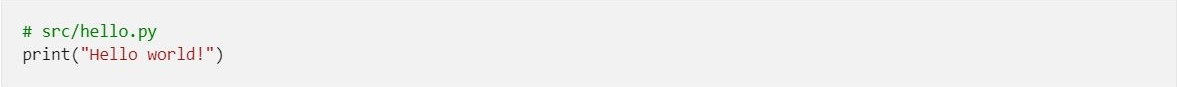
\includegraphics[scale=.1]{./Fig/hello.jpg}
    \end{frame}

    \begin{frame}
        \frametitle{Progress report}

        \begin{block}{\href{https://docs.microsoft.com/en-us/azure/machine-learning/tutorial-1st-experiment-hello-world}{hello.py}}
            \centering
            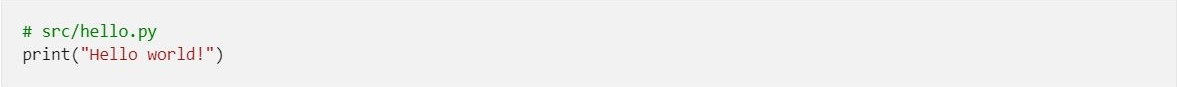
\includegraphics[width=4.5in]{./Fig/hello.jpg}
        \end{block}

        \begin{block}{\href{https://docs.microsoft.com/en-us/azure/machine-learning/tutorial-1st-experiment-hello-world}{run-hello.py}}
            \centering
            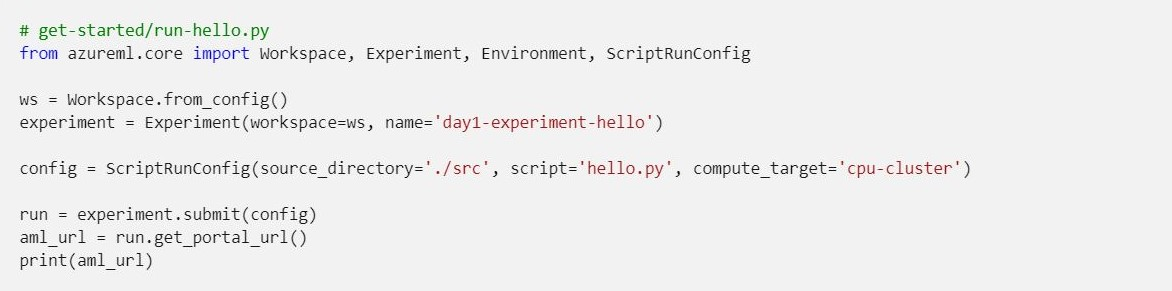
\includegraphics[width=4.5in]{./Fig/run_hello.jpg}
        \end{block}
    \end{frame}

\end{document}
